% Created by tikzDevice version 0.8.1 on 2015-11-20 15:35:03
% !TEX encoding = UTF-8 Unicode
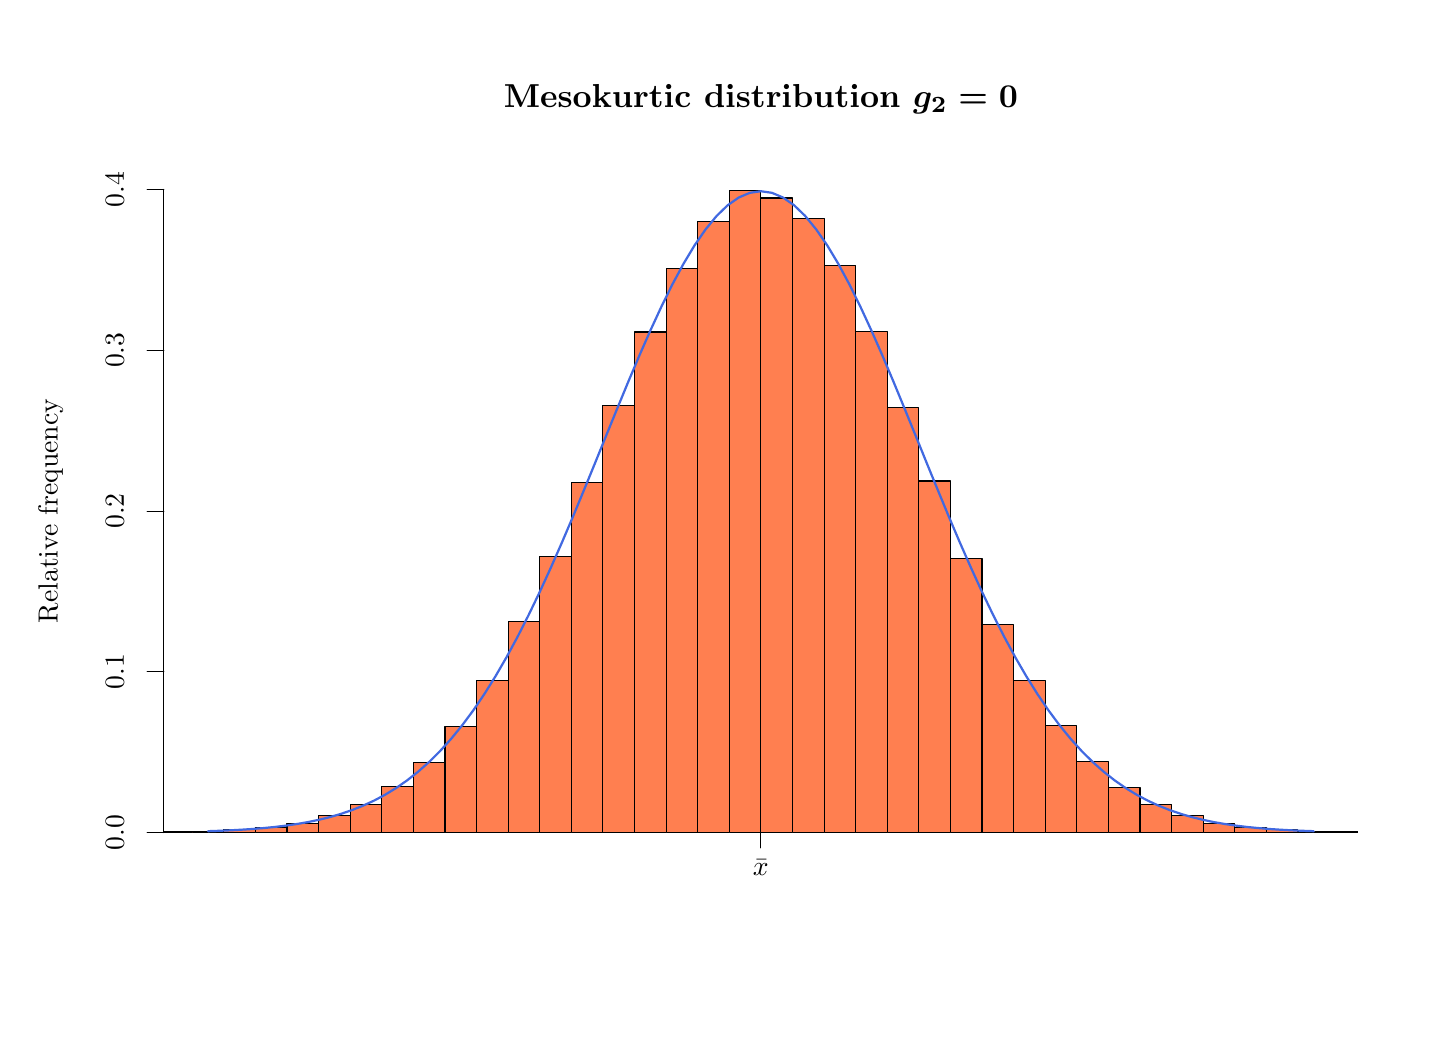
\begin{tikzpicture}[x=1pt,y=1pt]
\definecolor{fillColor}{RGB}{255,255,255}
\path[use as bounding box,fill=fillColor,fill opacity=0.00] (0,0) rectangle (505.89,361.35);
\begin{scope}
\path[clip] (  0.00,  0.00) rectangle (505.89,361.35);
\definecolor{drawColor}{RGB}{0,0,0}

\node[text=drawColor,anchor=base,inner sep=0pt, outer sep=0pt, scale=  1.20, font=\boldmath] at (264.94,332.61)
{\bfseries Mesokurtic distribution $g_2=0$};

\node[text=drawColor,rotate= 90.00,anchor=base,inner sep=0pt, outer sep=0pt, scale=  1.00] at ( 10.80,186.67) {Relative frequency};
\end{scope}
\begin{scope}
\path[clip] ( 49.20, 61.20) rectangle (480.69,312.15);
\definecolor{drawColor}{RGB}{0,0,0}
\definecolor{fillColor}{RGB}{255,127,80}

\path[draw=drawColor,line width= 0.4pt,line join=round,line cap=round,fill=fillColor] ( -9.02, 70.49) rectangle (  2.40, 70.50);

\path[draw=drawColor,line width= 0.4pt,line join=round,line cap=round,fill=fillColor] (  2.40, 70.49) rectangle ( 13.81, 70.50);

\path[draw=drawColor,line width= 0.4pt,line join=round,line cap=round,fill=fillColor] ( 13.81, 70.49) rectangle ( 25.23, 70.51);

\path[draw=drawColor,line width= 0.4pt,line join=round,line cap=round,fill=fillColor] ( 25.23, 70.49) rectangle ( 36.64, 70.54);

\path[draw=drawColor,line width= 0.4pt,line join=round,line cap=round,fill=fillColor] ( 36.64, 70.49) rectangle ( 48.06, 70.59);

\path[draw=drawColor,line width= 0.4pt,line join=round,line cap=round,fill=fillColor] ( 48.06, 70.49) rectangle ( 59.47, 70.76);

\path[draw=drawColor,line width= 0.4pt,line join=round,line cap=round,fill=fillColor] ( 59.47, 70.49) rectangle ( 70.89, 71.04);

\path[draw=drawColor,line width= 0.4pt,line join=round,line cap=round,fill=fillColor] ( 70.89, 70.49) rectangle ( 82.30, 71.48);

\path[draw=drawColor,line width= 0.4pt,line join=round,line cap=round,fill=fillColor] ( 82.30, 70.49) rectangle ( 93.72, 72.39);

\path[draw=drawColor,line width= 0.4pt,line join=round,line cap=round,fill=fillColor] ( 93.72, 70.49) rectangle (105.13, 73.87);

\path[draw=drawColor,line width= 0.4pt,line join=round,line cap=round,fill=fillColor] (105.13, 70.49) rectangle (116.55, 76.63);

\path[draw=drawColor,line width= 0.4pt,line join=round,line cap=round,fill=fillColor] (116.55, 70.49) rectangle (127.96, 80.62);

\path[draw=drawColor,line width= 0.4pt,line join=round,line cap=round,fill=fillColor] (127.96, 70.49) rectangle (139.38, 87.11);

\path[draw=drawColor,line width= 0.4pt,line join=round,line cap=round,fill=fillColor] (139.38, 70.49) rectangle (150.79, 95.88);

\path[draw=drawColor,line width= 0.4pt,line join=round,line cap=round,fill=fillColor] (150.79, 70.49) rectangle (162.21,108.91);

\path[draw=drawColor,line width= 0.4pt,line join=round,line cap=round,fill=fillColor] (162.21, 70.49) rectangle (173.62,125.60);

\path[draw=drawColor,line width= 0.4pt,line join=round,line cap=round,fill=fillColor] (173.62, 70.49) rectangle (185.04,146.75);

\path[draw=drawColor,line width= 0.4pt,line join=round,line cap=round,fill=fillColor] (185.04, 70.49) rectangle (196.45,170.20);

\path[draw=drawColor,line width= 0.4pt,line join=round,line cap=round,fill=fillColor] (196.45, 70.49) rectangle (207.87,197.01);

\path[draw=drawColor,line width= 0.4pt,line join=round,line cap=round,fill=fillColor] (207.87, 70.49) rectangle (219.28,224.77);

\path[draw=drawColor,line width= 0.4pt,line join=round,line cap=round,fill=fillColor] (219.28, 70.49) rectangle (230.70,251.37);

\path[draw=drawColor,line width= 0.4pt,line join=round,line cap=round,fill=fillColor] (230.70, 70.49) rectangle (242.11,274.44);

\path[draw=drawColor,line width= 0.4pt,line join=round,line cap=round,fill=fillColor] (242.11, 70.49) rectangle (253.53,291.16);

\path[draw=drawColor,line width= 0.4pt,line join=round,line cap=round,fill=fillColor] (253.53, 70.49) rectangle (264.94,302.52);

\path[draw=drawColor,line width= 0.4pt,line join=round,line cap=round,fill=fillColor] (264.94, 70.49) rectangle (276.36,299.78);

\path[draw=drawColor,line width= 0.4pt,line join=round,line cap=round,fill=fillColor] (276.36, 70.49) rectangle (287.78,292.37);

\path[draw=drawColor,line width= 0.4pt,line join=round,line cap=round,fill=fillColor] (287.78, 70.49) rectangle (299.19,275.50);

\path[draw=drawColor,line width= 0.4pt,line join=round,line cap=round,fill=fillColor] (299.19, 70.49) rectangle (310.61,251.48);

\path[draw=drawColor,line width= 0.4pt,line join=round,line cap=round,fill=fillColor] (310.61, 70.49) rectangle (322.02,224.09);

\path[draw=drawColor,line width= 0.4pt,line join=round,line cap=round,fill=fillColor] (322.02, 70.49) rectangle (333.44,197.54);

\path[draw=drawColor,line width= 0.4pt,line join=round,line cap=round,fill=fillColor] (333.44, 70.49) rectangle (344.85,169.59);

\path[draw=drawColor,line width= 0.4pt,line join=round,line cap=round,fill=fillColor] (344.85, 70.49) rectangle (356.27,145.54);

\path[draw=drawColor,line width= 0.4pt,line join=round,line cap=round,fill=fillColor] (356.27, 70.49) rectangle (367.68,125.35);

\path[draw=drawColor,line width= 0.4pt,line join=round,line cap=round,fill=fillColor] (367.68, 70.49) rectangle (379.10,109.13);

\path[draw=drawColor,line width= 0.4pt,line join=round,line cap=round,fill=fillColor] (379.10, 70.49) rectangle (390.51, 96.33);

\path[draw=drawColor,line width= 0.4pt,line join=round,line cap=round,fill=fillColor] (390.51, 70.49) rectangle (401.93, 86.82);

\path[draw=drawColor,line width= 0.4pt,line join=round,line cap=round,fill=fillColor] (401.93, 70.49) rectangle (413.34, 80.76);

\path[draw=drawColor,line width= 0.4pt,line join=round,line cap=round,fill=fillColor] (413.34, 70.49) rectangle (424.76, 76.70);

\path[draw=drawColor,line width= 0.4pt,line join=round,line cap=round,fill=fillColor] (424.76, 70.49) rectangle (436.17, 73.85);

\path[draw=drawColor,line width= 0.4pt,line join=round,line cap=round,fill=fillColor] (436.17, 70.49) rectangle (447.59, 72.34);

\path[draw=drawColor,line width= 0.4pt,line join=round,line cap=round,fill=fillColor] (447.59, 70.49) rectangle (459.00, 71.51);

\path[draw=drawColor,line width= 0.4pt,line join=round,line cap=round,fill=fillColor] (459.00, 70.49) rectangle (470.42, 70.99);

\path[draw=drawColor,line width= 0.4pt,line join=round,line cap=round,fill=fillColor] (470.42, 70.49) rectangle (481.83, 70.76);

\path[draw=drawColor,line width= 0.4pt,line join=round,line cap=round,fill=fillColor] (481.83, 70.49) rectangle (493.25, 70.62);

\path[draw=drawColor,line width= 0.4pt,line join=round,line cap=round,fill=fillColor] (493.25, 70.49) rectangle (504.66, 70.53);

\path[draw=drawColor,line width= 0.4pt,line join=round,line cap=round,fill=fillColor] (504.66, 70.49) rectangle (516.08, 70.52);
\end{scope}
\begin{scope}
\path[clip] (  0.00,  0.00) rectangle (505.89,361.35);
\definecolor{drawColor}{RGB}{0,0,0}

\path[draw=drawColor,line width= 0.4pt,line join=round,line cap=round] (264.92, 70.49) -- (264.92, 65);

\node[text=drawColor,anchor=base,inner sep=0pt, outer sep=0pt, scale=  1.00] at (264.92, 55) {$\bar x$};

\path[draw=drawColor,line width= 0.4pt,line join=round,line cap=round] ( 49.20, 70.49) -- ( 49.20,302.86);

\path[draw=drawColor,line width= 0.4pt,line join=round,line cap=round] ( 49.20, 70.49) -- ( 43.20, 70.49);

\path[draw=drawColor,line width= 0.4pt,line join=round,line cap=round] ( 49.20,128.58) -- ( 43.20,128.58);

\path[draw=drawColor,line width= 0.4pt,line join=round,line cap=round] ( 49.20,186.67) -- ( 43.20,186.67);

\path[draw=drawColor,line width= 0.4pt,line join=round,line cap=round] ( 49.20,244.77) -- ( 43.20,244.77);

\path[draw=drawColor,line width= 0.4pt,line join=round,line cap=round] ( 49.20,302.86) -- ( 43.20,302.86);

\node[text=drawColor,rotate= 90.00,anchor=base,inner sep=0pt, outer sep=0pt, scale=  1.00] at ( 34.80, 70.49) {0.0};

\node[text=drawColor,rotate= 90.00,anchor=base,inner sep=0pt, outer sep=0pt, scale=  1.00] at ( 34.80,128.58) {0.1};

\node[text=drawColor,rotate= 90.00,anchor=base,inner sep=0pt, outer sep=0pt, scale=  1.00] at ( 34.80,186.67) {0.2};

\node[text=drawColor,rotate= 90.00,anchor=base,inner sep=0pt, outer sep=0pt, scale=  1.00] at ( 34.80,244.77) {0.3};

\node[text=drawColor,rotate= 90.00,anchor=base,inner sep=0pt, outer sep=0pt, scale=  1.00] at ( 34.80,302.86) {0.4};
\end{scope}
\begin{scope}
\path[clip] ( 49.20, 61.20) rectangle (480.69,312.15);
\definecolor{drawColor}{RGB}{65,105,225}

\path[draw=drawColor,line width= 0.8pt,line join=round,line cap=round] ( 65.18, 71.00) --
	( 69.18, 71.14) --
	( 73.17, 71.31) --
	( 77.17, 71.53) --
	( 81.16, 71.79) --
	( 85.16, 72.12) --
	( 89.15, 72.51) --
	( 93.15, 72.99) --
	( 97.14, 73.57) --
	(101.14, 74.26) --
	(105.13, 75.09) --
	(109.13, 76.07) --
	(113.12, 77.23) --
	(117.12, 78.59) --
	(121.11, 80.18) --
	(125.11, 82.02) --
	(129.11, 84.14) --
	(133.10, 86.57) --
	(137.10, 89.35) --
	(141.09, 92.50) --
	(145.09, 96.04) --
	(149.08,100.02) --
	(153.08,104.44) --
	(157.07,109.34) --
	(161.07,114.73) --
	(165.06,120.61) --
	(169.06,127.01) --
	(173.05,133.90) --
	(177.05,141.29) --
	(181.04,149.16) --
	(185.04,157.47) --
	(189.03,166.19) --
	(193.03,175.27) --
	(197.03,184.65) --
	(201.02,194.27) --
	(205.02,204.03) --
	(209.01,213.87) --
	(213.01,223.67) --
	(217.00,233.35) --
	(221.00,242.79) --
	(224.99,251.88) --
	(228.99,260.53) --
	(232.98,268.61) --
	(236.98,276.03) --
	(240.97,282.68) --
	(244.97,288.47) --
	(248.96,293.33) --
	(252.96,297.19) --
	(256.95,299.98) --
	(260.95,301.67) --
	(264.94,302.24) --
	(268.94,301.67) --
	(272.94,299.98) --
	(276.93,297.19) --
	(280.93,293.33) --
	(284.92,288.47) --
	(288.92,282.68) --
	(292.91,276.03) --
	(296.91,268.61) --
	(300.90,260.53) --
	(304.90,251.88) --
	(308.89,242.79) --
	(312.89,233.35) --
	(316.88,223.67) --
	(320.88,213.87) --
	(324.87,204.03) --
	(328.87,194.27) --
	(332.86,184.65) --
	(336.86,175.27) --
	(340.86,166.19) --
	(344.85,157.47) --
	(348.85,149.16) --
	(352.84,141.29) --
	(356.84,133.90) --
	(360.83,127.01) --
	(364.83,120.61) --
	(368.82,114.73) --
	(372.82,109.34) --
	(376.81,104.44) --
	(380.81,100.02) --
	(384.80, 96.04) --
	(388.80, 92.50) --
	(392.79, 89.35) --
	(396.79, 86.57) --
	(400.78, 84.14) --
	(404.78, 82.02) --
	(408.77, 80.18) --
	(412.77, 78.59) --
	(416.77, 77.23) --
	(420.76, 76.07) --
	(424.76, 75.09) --
	(428.75, 74.26) --
	(432.75, 73.57) --
	(436.74, 72.99) --
	(440.74, 72.51) --
	(444.73, 72.12) --
	(448.73, 71.79) --
	(452.72, 71.53) --
	(456.72, 71.31) --
	(460.71, 71.14) --
	(464.71, 71.00);
\end{scope}
\end{tikzpicture}
